	\section{Wstęp} 
		\par Niniejszy dokument przedstawia biznes plan sklepu internetowego. Zawiera on opis wszystkich narzędzi niezbędnych do zarządzania i funkcjonowania takiego sklepu. Znajdziemy tu: plan finansowy i rozwojowy; analizę rynków sprzedaży w Polsce i Kanadzie; analizę branży meblarskiej; szczegółowe informacje na temat sprzętu niezbędnego do prowadzenia bezpiecznego i wydajnego sklepu internetowego. W dokumencie znalazły się także regulaminy w języku angielskim i polskim; karty gwarancyjne; informacje dotyczące polityki cookies. 
	
		\par Dokument ten, powstał z chęci przybliżenia zagadnień związanych z funkcjonowaniem coraz popularniejszych sklepów internetowych. Skupia się on na branży meblarskiej, która rokrocznie zwiększa swoje udziały w rynku. Sklep jaki pragnę stworzyć będzie zrzeszać niewielkich rzemieślników , fachowców mogących sprostać oczekiwaniom coraz bardziej wymagających klientów.
	
	\section{Specyfikacja przedsiębiorstwa}
		\begin{description}
			\item Data rozpoczęcia działalności - 01.06.2017
			\item Rodzaj działalności - handel
			\item Zakres działalności - PKD 47.91.Z  Sprzedaż detaliczna prowadzona przez domy sprzedaży wysyłkowej lub Internet	
			\item Sprzedaż produktów - rejestrowana za pomocą kasy fiskalnej
			\item Rozliczenie podatku dochodowego - książka przychodów i rozchodów
			\item Rozliczenie podatku VAT - podatnik Vat
		\end{description}
	
	\section{Wykształcenie; doświadczenie zawodowe; szkolenia}
	\subsection{Wykształcenie}
		\begin{itemize}
			\item 2008-2014 Wyższa Szkoła Zarządzania Edukacja; kierunek „Dziennikarstwo i komunikacja społeczna”
         \item 2000-2004 III Liceum Ogólnokształcące w Świdnicy 
		\end{itemize}
		
	\subsection{Doświadczenie zawodowe}
		\begin{itemize}
			\item 1.03.2012 - 31.10.2016 Kazar Footwear Sp. z o.o. - handlowiec/menadżer
			\item 20.02.2008 - 31.05.2011 Wittchen S.A. - sprzedawca, kierownik
			\item 27.03.2007 - 18.06.2007 Reserved LPP S.A. - sprzedawca  
		\end{itemize}	
		
	\subsection{Przebyte szkolenia}
		\begin{itemize}
			\item szkolenia w ramach projektu unijnego: księgowość, kadry i płace, ABC przedsiębiorczości, biznes plan,  ubezpieczenia społeczne, prawo podatkowe
			\item szkolenie dla kadry kierowniczej z zakresu BHP
			\item szkolenia wewnętrzne w firmach z zakresu zarządzania, technik sprzedaży, marketingu
		\end{itemize}
		
	\section{Podstawowe cele działalności}
		\par Głównym celem planowanej działalności gospodarczej, będzie internetowa działalność handlowa w branży meblowej. Określana także mianem działalności e-commerce w branży meblowej. Będzie ona skupiać się na sprzedaży eksportowej mebli pochodzących od małych i średnich producentów z Polski na teren Kanady, jak i na sprzedaży na rynku polskim. Główne nakłady pracy skupione będą na eksporcie ze względu na dochodowość tego rynku.
			
		\par Przedmiotem handlu na terytorium Polski i Kanady będą meble domowe. Handel odbywać będzie się poprzez portale aukcyjne i sklep internetowy. Zarówno obsługa ogłoszeń jak i sklepu internetowego będzie przebiegać w języku polskim i angielskim. Procesy jakie należy wykonać to: proces obsługi klienta, proces reklamacji, proces promocji. W procesie obsługi klienta składający zamówienie będą mieli możliwość dostosowania produktu do swoich potrzeb. Produkt prezentowany na stronie internetowej lub ogłoszeniu, to jedynie wzór produktu do wykonania. Dla tak skonfigurowanego produktu utworzone zostanie zlecenie produkcji. Produkt zostanie wykonany przez producenta według zamówienia i dostarczony do klienta. W procesie reklamacji należy przyjąć lub odrzucić zgłoszenie klienta oraz podjąć działania zmierzające do wyeliminowania wad produktu lub odrzucenia roszczeń. 
			
		\par Prowadzenie tego typu działalności wymaga wykonywania określonych zadań, do których należy obsługa klientów i producentów, promocja sklepu, sporządzanie statystyk.  Jak również pozyskanie środków sprzętowych, celem wprowadzenia odpowiedniej organizacji tych zadań. Koncept działalności przestawia następująca mapa:
			
		\begin{figure}[H]
			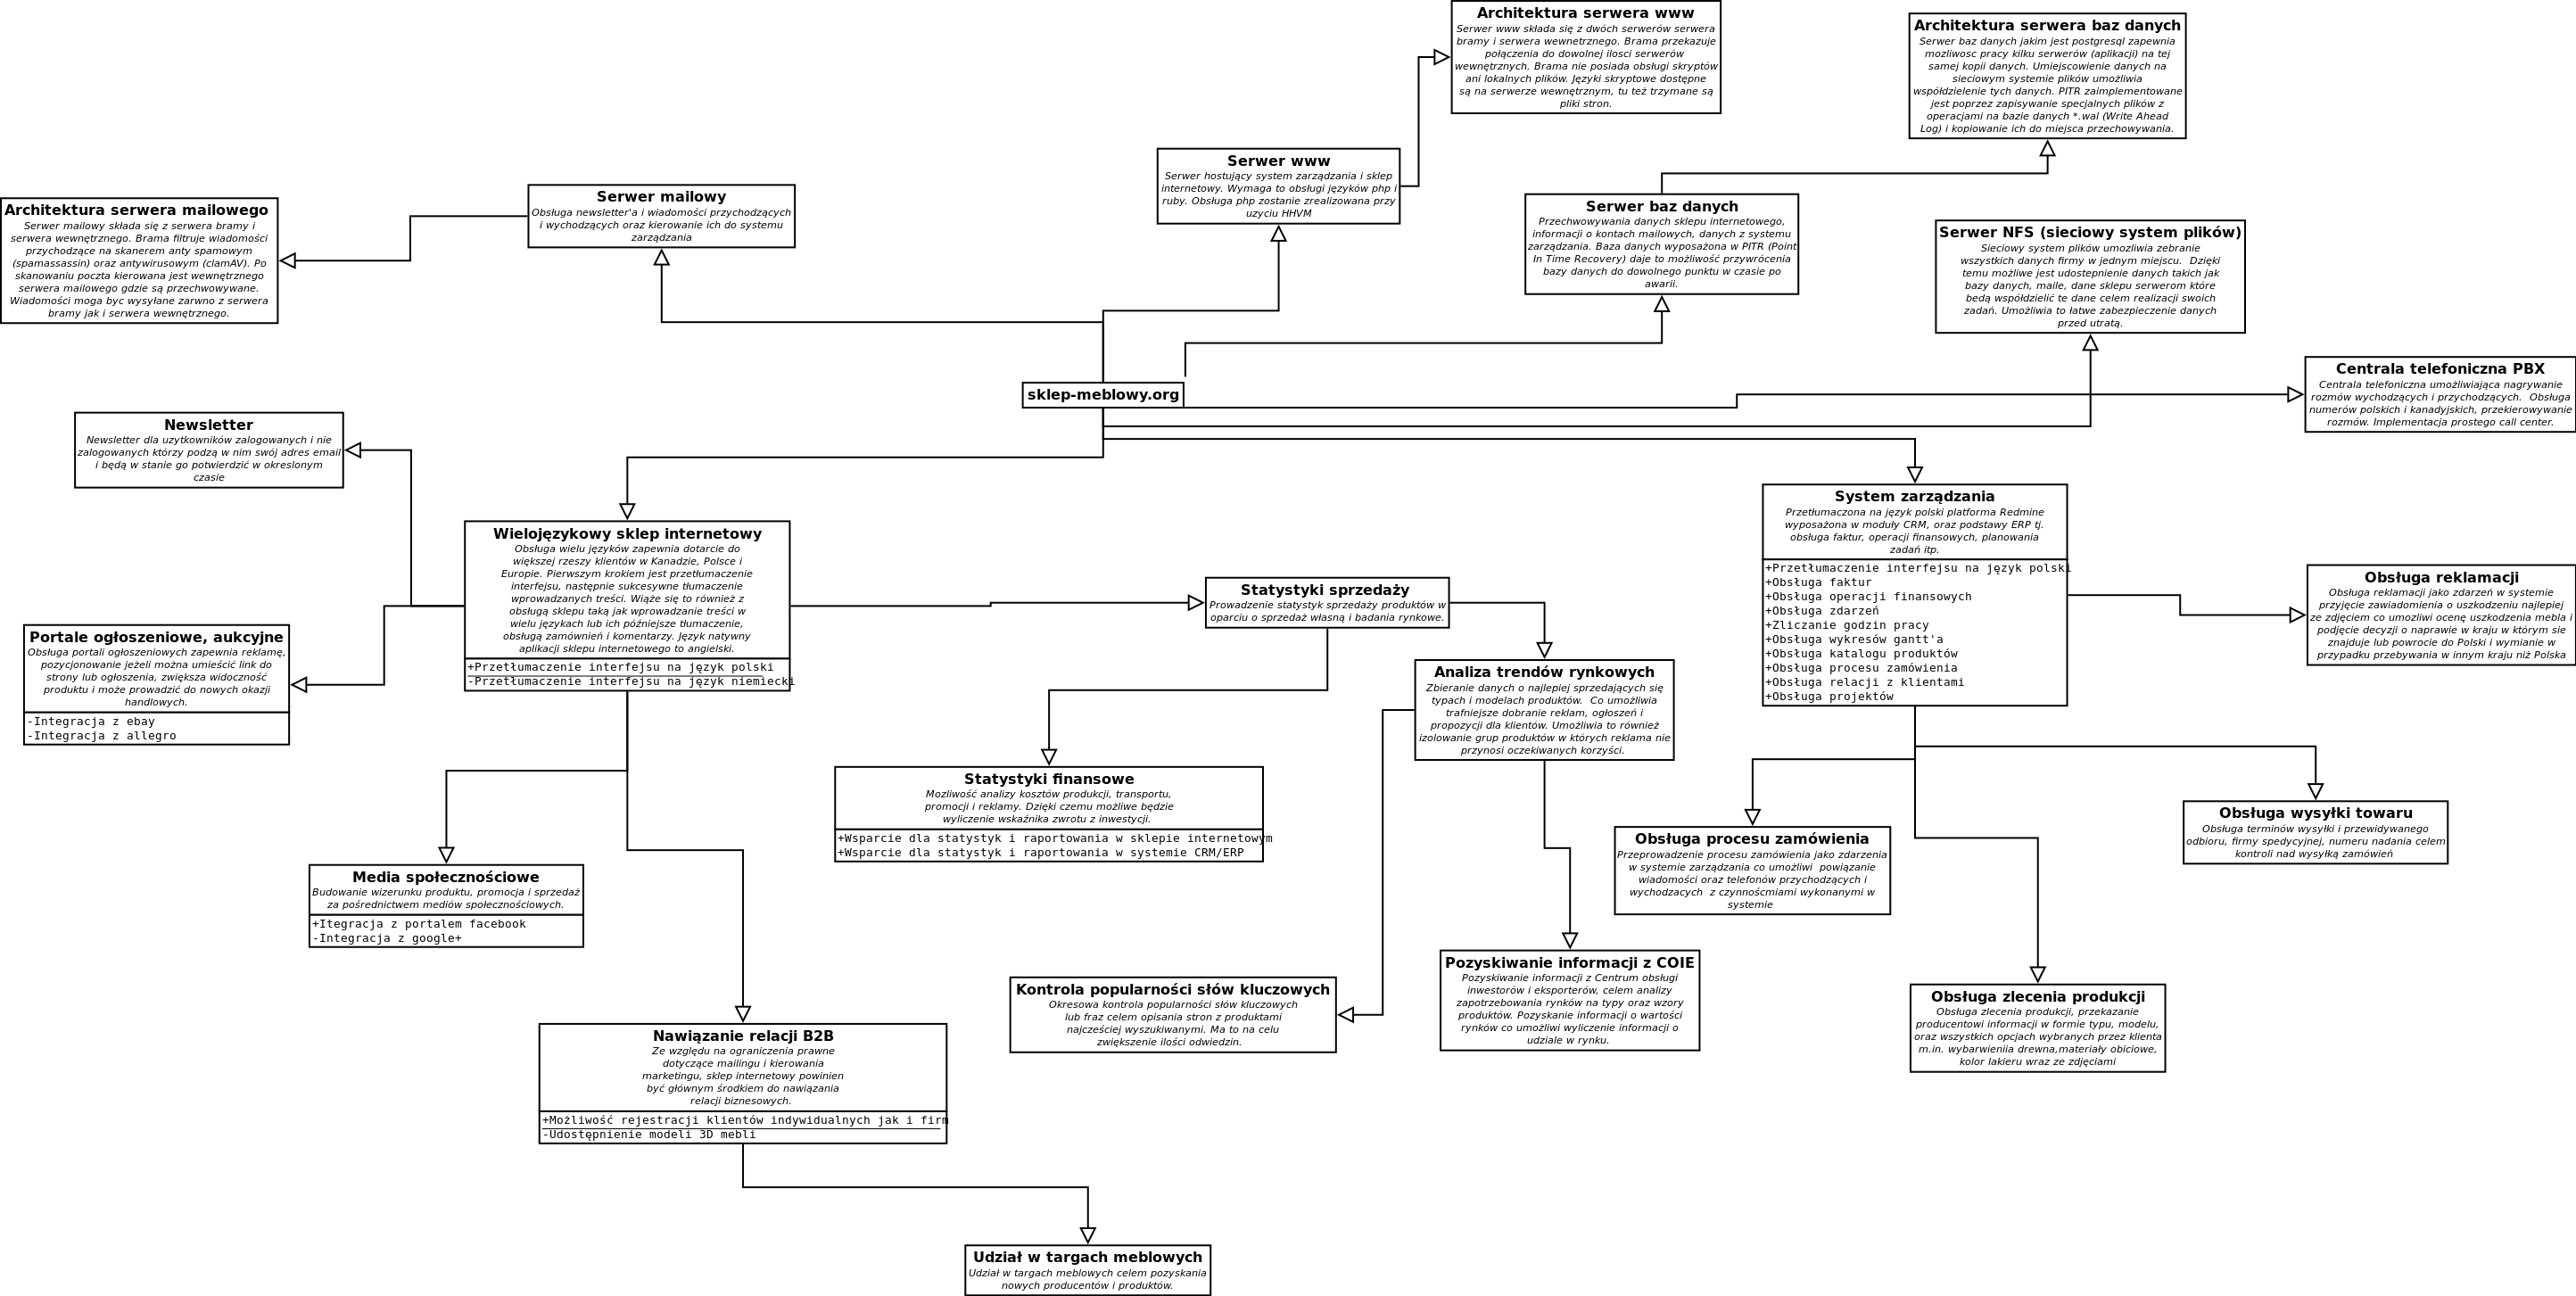
\includegraphics[scale=0.25,angle=90]{mindmap}
			\caption{Mapa projektu przedstawiająca konspekt środków, zadań i organizacji}
		\end{figure}
		
	\section{Oferowane usługi}
		\subsubsection{Usługa sprzedaży} 
			\par Przedmiotem podejmowanej działalności będzie internetowy sklep meblowy, oferujący sprzedaż asortymentu polskich wytwórców meblowych na rynku polskim jak i rynkach zagranicznych (ze szczególnym uwzględnieniem Kanady). Głównym produktem będą meble drewniane i tapicerowane. Po analizie rynku udało się ustalić, że przewagą mebli produkowanych w Polsce jest ich wysoka jakość oraz niska cena. Planuje być przede wszystkim pośrednikiem między wymagającymi, szukającymi wysokiej jakości klientami, a producentami tych dóbr, którzy w dużej mierze sami nie potrafią przebić się na szeroki rynek zbytu lub mają zbyt mały budżet na organizację kampanii reklamowej.
				
			\par Na stronie internetowej znajdować się będą istniejące wzory mebli od producentów wraz z możliwością ich dostosowania pod indywidualne wymagania klienta. Kluczowe jest więc zebranie jak największej liczby materiałów obiciowych, rodzajów drewna i jego wybarwień, okuć itp. tak, aby klient miał możliwość wpływu na powstanie produktu. Taki zabieg daje jeszcze jedną przewagę zarówno w świetle polskiego jak i kanadyjskiego prawa, ponieważ nie ma możliwości zwrotu towaru mocno spersonalizowanego.
				
		\subsubsection{Usługa reklamacji} 
			\par Drugą oferowaną usługą jest proces reklamacji. Usługa ta przeznaczona będzie dla klientów, u których wystąpią wady produktu w trakcie użytkowania lub produkt będzie niezgodny z zamówieniem. Na proces reklamacji składać się będzie przesłanie zdjęć wadliwego towaru przez klienta. Na podstawie tych zdjęć musi nastąpić decyzja o uznaniu lub odrzuceniu reklamacji. W przypadku uznania reklamacji w Polsce, należy zwrócić towar do producenta celem wykonania  niezbędnych napraw. W przypadku sprzedaży zagranicznej naprawa musi zostać wykonana na miejscu, co może wiązać się z koniecznością dosłania części zamiennych. Jeżeli naprawa nie jest możliwa na miejscu, produkt zostanie zwrócony do producenta lub wymieniony (w wypadku gdy koszty logistyki od klienta do producenta i z powrotem przekroczą wartość produktu).

	\section{Charakterystyka produktów}
		\par Moim celem jest zaprezentowanie produktów pochodzących od polskich producentów mebli, których wyróżnia jakość  użytych materiałów, dbałość o szczegóły i bardzo dobre wykonanie. Zależy mi aby wyjść naprzeciw oczekiwaniom współczesnego klienta, któremu co raz częściej zależy na produkcie mocno zindywidualizowanym. Dlatego klient sam będzie mógł dobrać sobie atrybuty produktu. Sprzedawanymi produktami będą meble domowe, w skład których wchodzą: 
	
		\begin{itemize}
			\item{sofy}
                \begin{itemize}
                    \item skórzane
                    \item tapicerowane
                    \item rozkładane
                    \item narożniki
                \end{itemize}
				
				\item{fotele}
					\begin{itemize}
					\item obrotowe
					\item skórzane
					\item tapicerowane
					\item z podnóżkiem
					\end{itemize}
					
            \item{łóżka}
                \begin{itemize}
                    \item drewniane
                    \item tapicerowane
                    \item podwójne
                    \item pojedyncze
                \end{itemize}
					
            \item{krzesła}
                \begin{itemize}
                    \item drewniane
                    \item obrotowe
                    \item biurowe
                    \item skórzane
                    \item hokery
                \end{itemize}
					
				\item{stoły}
                \begin{itemize}
                    \item drewniane
                    \item wysoki połysk
                    \item szklane
                    \item okrągłe
                \end{itemize}
					
				\item{stoliki kawowe}
                \begin{itemize}
                    \item drewniane
                    \item wysoki połysk
                    \item okrągłe
                    \item prostokątne
                \end{itemize}
					
				\item{szafki nocne}
                \begin{itemize}
                    \item drewniane
                    \item wysoki połysk
                \end{itemize}
					
				\item{szafki RTV}
                \begin{itemize}
                    \item drewniane
                    \item wysoki połysk
                    \item wiszące
                    \item stojące
                \end{itemize}
					
            \item{regały}
                \begin{itemize}
                    \item drewniane
                    \item wysoki połysk
                    \item stojące
                    \item wiszące
                \end{itemize}
				
            \item{biurka}
                \begin{itemize}
                    \item drewniane
                    \item wysoki połysk
                \end{itemize}
				
            \item{komody}
                \begin{itemize}
                    \item drewniane
                    \item wysoki połysk
                    \item niskie
                    \item wysokie
                \end{itemize}
		\end{itemize}
	
		\par Meble mogą być wykonane lub posiadać wykończenie z różnych materiałów. Poniżej zaprezentowane zostaną materiały, z których mogą być wykonane meble:
		
		\begin{itemize}
			\item{Drewno i płyty drewniane}
				\begin{itemize}
					\item{Drewno sosnowe} - jest sprężyste, wytrzymałe, posiada kremowe, szerokie usłojenie
					\item{Drewno bukowe} - należy do drzew długowiecznych ,jest twarde, ścisłe, znosi duże obciążenia
					\item{Drewno dębowe} - jest ciężkie, wytrzymałe, twarde, odporne na ścieranie
					\item{Drewno jesionowe} - jest ciężkie, twarde i sprężyste
					\item{Drewno olchowe} - średnio twarde, idealne do obróbki
				\end{itemize}
			\item{Płyty drewnopochodne}
				\begin{itemize}
					\item{płyty pilśniowe} - Powstają one ze sprasowanej rozwłóknionej masy drzewnej dzielą się one względem gęstości
						\begin{itemize}
							\item{MDF} - płyta o średniej gęstości
							\item{HDF} - płyta o wysokiej gęstości
							\item{LDF} - płyta o niskiej gęstości
						\end{itemize}
					\item{płyty wiórowe} produkowane z wiórów drzewnych sklejanych klejami syntetycznymi
					\item{płyty paździerzowe} są najmniej szlachetną odmianą płyt drewnopochodnych - powstają ze spojenia klejem zdrewniałych łodyg roślin
				\end{itemize}
		\end{itemize}
		
		\par Materiały obiciowe dzielimy na:
		
		\begin{itemize}	
			\item{materiały}
				\begin{itemize}
					\item{Altary,alcantary} - cechuje je miękka struktura odporna na ścieranie
					\item{Floki} - materiał przypominający nubuk, posiada wysoką żywotność
					\item{Mikrofazy} - mają niską cenę, wysoką elastyczność i żywotność
					\item{Plusze} - wyróżniamy-aksamity, welury i welwety. Mają dużą wytrzymałość i są miłe w dotyku.
					\item{Szenile} - łatwe w utrzymaniu, mają duża wytrzymałość i odporność
				\end{itemize}
			\item{skóry}
				\begin{itemize}
					\item{Skóra gładka z warstwą pigmentu} - barwiona powierzchniowo, łatwa w czyszczeniu i pielęgnacji
					\item{Skóra anilinowa} - o otwartych porach, wrażliwa ,trudna w utrzymaniu ale najwyższej klasy
					\item{Skóra zamszowa, nubukowa} - skóra otwarta,zeszlifowana
				\end{itemize}
		\end{itemize}
			
		\par Materiały, z których najczęściej wykonuje się dane meble:
		\begin{itemize}
			\item{stoły, biurka} - buk,dąb, sosna,brzoza
			\item{łóżka} - dąb,brzoza,jesion,sosna,buk
			\item{krzesła} - dąb, sosna, buk
		\end{itemize}
		
	\section{Motywy podjęcia działalności}
		\subsection{Doświadczenie i motywacja}
			\par Od 10 lat zajmuję się handlem, co pozwoliło mi na zdobycie niezbędnego doświadczenia i praktycznej wiedzy. Dzięki ciężkiej pracy, dwukrotnie awansowałam na stanowisko menadżera. Przeszłam szereg szkoleń, począwszy od technik sprzedaży, efektywnej organizacji czasu pracy, jak i podstaw marketingu. Pracowałam z systemami kontroli i zarządzania pracą, systemami kasowymi itp. Dzięki pracy w firmach handlowych nabyłam wiedzę organizacyjną i podstawy wiedzy technicznej związanej z organizacją sprzedaży. 

			\par Zdecydowałam się na branżę meblarską, ponieważ od długiego czasu obserwuje wzrost zainteresowania produktami niepowtarzalnymi, oryginalnymi, które wychodzą spod rąk rzemieślnika a nie taśmy. W Polsce posiadamy znakomitych wytwórców, którzy doskonale łączą współczesne trendy i wysoką jakość. Są oni doceniani zarówno w Polsce jak i zagranicą. Mimo bardzo dobrych jakościowo mebli polscy producenci wciąż otrzymują za nie bardzo niską cenę. Taki stan rzeczy wiążę się z głównie ze sprzedażą produktów na rynku hurtowym, oraz produkcji dla sieci takich jak "IKEA". Brak jest na rynku polskim dystrybutorów detalicznych, gotowych podjąć wyzwanie sprzedaży międzynarodowej. Sytuację tą obrazuje wykres przedstawiający cenę mebli za tonę produktu w dolarach amerykańskich. Wedle tego wykresu otrzymujemy za tonę produktu najmniej z czołowych producentów.
			
			\begin{figure}[H]
				\centering
				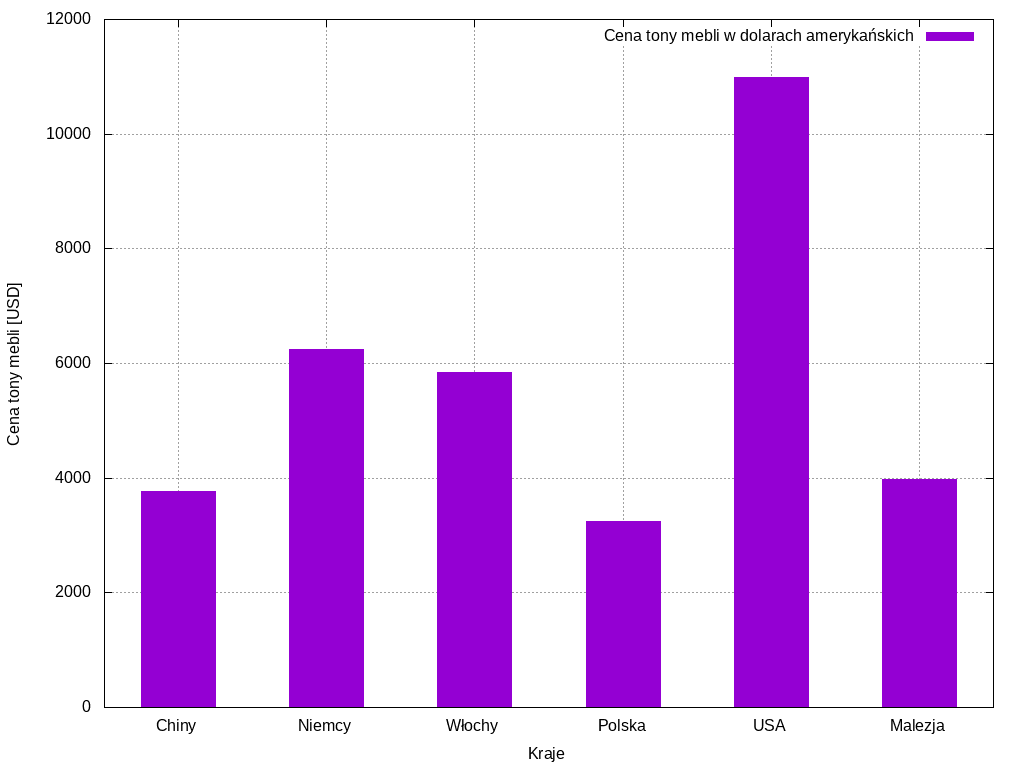
\includegraphics[scale=0.45]{price_weight}
				\caption{Wykres przedstawiający cenę za tonę mebli w danym państwie}
			\end{figure}
		
		\subsection{Uzasadnienie wyboru branży}
			\par Rynek e-commerce w Polsce z roku na rok notuje coraz lepsze wyniki. Według badań przeprowadzonych przez Gemius, prawie połowa Polaków robi zakupy przez internet. W ich opinii zakupy on-line są wygodniejsze, tańsze, dostępne całą dobę, dają możliwość większego wyboru produktów. Wedle informacji zawartych w sprawozdaniu "Handel internetowy w Polsce 2015, analiza prognoza rozwoju rynku e-commerce  na lata 2015-2020", e-handel notuje stabilną dynamikę wzrostu, niezależnie od sytuacji na całym rynku detalicznym.
			Polska jest również jednym z największych na świecie eksporterów mebli, a polska branża meblarska notuje zyski rok po roku, zarówno na rynku internetowym jak i stacjonarnym. Polscy producenci posiadają dobrą renomę  na rynkach eksportowych. Według analizy B+R Studio i Ogólnopolskiej Izby Gospodarczej Producentów Mebli, eksport polskich mebli w 2016 roku przekroczył 40 mld złotych. Rokrocznie wzrasta na poziomie 10 procent. Polskie produkty są cenione nie tylko za konkurencyjne ceny, ale również za solidne wykonanie, użyte materiały i design. 
		
			\begin{figure}[H]
				\centering
				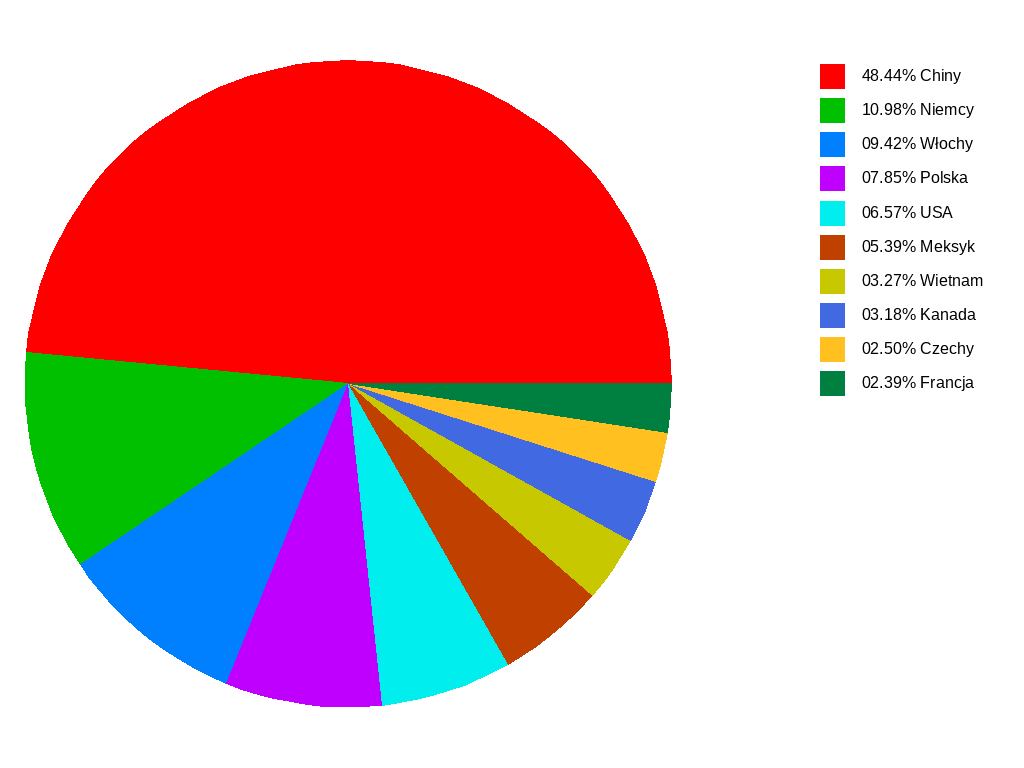
\includegraphics[scale=0.5]{export_swiat}
				\caption{Wykres przedstawiający procentowy udział czołowych krajów w rynku eksportowym}
			\end{figure}
	
		\subsection{Motywacje osobiste}
			\par Nadrzędną motywacją, która skłoniła mnie do próby podjęcia tego przedsięwzięcia, jest moje długoletnie doświadczenie w handlu i sukcesy z nią związane. Do tej pory działałam na rynku polskim, a jako osoba ambitna, chcę również sprawdzić swoje możliwości w handlu międzynarodowym. Dlatego też od dłuższego czasu obserwowałam skale sprzedaży na rynkach e-commerce. Ze względu na doświadczenie zawodowe i wykształcenie, posiadam obszerną wiedzę dotyczącą handlu jak i komunikacji społecznej. Dlatego wiem, że kluczową sprawą jest nie tylko bezpieczeństwo danych klientów, świetnie przygotowany sklep internetowy, ale również profesjonalna obsługa klienta
			\par Znaczącą motywacją było również pojawienie się kompleksowej umowy handlowo-gospodarczej "CETA", która usuwa konieczność opłacenia ceł, co upraszcza formalności i obniża koszty eksportu. 

	\section{Stan przygotowań do podjęcia działalności gospodarczej}
		\par W związku z planowanym przedsięwzięciem, podjęłam szereg działań umożliwiających mi szybsze rozpoczęcie pracy nad własnym sklepem. Na dzień dzisiejszy posiadam wiele narzędzi niezbędnych do działania sklepu internetowego. Są to kosztowne narzędzia programowe gwarantujące przede wszystkim niezależność, bezpieczeństwo sklepu jak i klientów, oraz nienaganne działanie platformy.

		\subsection{Posiadane środki}
			\paragraph{Organizacja firmy}
				\begin{itemize}
					\item Opracowany logotyp
					\item Zakupione domeny
						\begin{itemize}
							\item sklep-meblowy.org
							\item furniture-store.ca
						\end{itemize}
					\item oprogramowanie sklepu internetowego bazujące na platformie Drupal
						\begin{itemize}
							\item Tworzenie kont indywidualnych dla klientów;
							\item Tworzenie profili biznesowych dla kontrahentów;
							\item Dodawanie produktów ze zdjęciami;
							\item Wielojęzyczność;
							\item Przeliczanie walut;
							\item Przyjazny interfejs wraz z możliwością edycji;
							\item Integracja z portalami społecznościowymi;
							\item Statystyki odwiedzin;
							\item Rozbudowana wyszukiwarka produktów;
							\item Kategoryzacja produktów na podstawie wyszukiwanych pozycji;
							\item Synchronizacja z systemem ERP;
							\item Ochrona przed spamem;
						\end{itemize}
					\item oprogramowanie serwera stron internetowych
						\begin{itemize}
							\item Obsługa strony internetowej; 
							\item Obsługa kopii strony. 
						\end{itemize}
					\item oprogramowanie serwera wiadomości e-mail
						\begin{itemize}
							\item Podpisywanie poczty wychodzącej;
							\item Wysyłanie załączników;
							\item Skanowanie antywirusowe;
							\item Filtrowanie spamu.
						\end{itemize}
					\item centrala telefoniczna PBX
						\begin{itemize}
							\item Nagrywanie rozmów
							\item Obsługa polskiego i kanadyjskiego numeru
							\item Przekierowywanie rozmów
						\end{itemize}
					\item system zarządzania bazujący na platformie Redmine
						\begin{itemize}
							\item Przechowywanie danych klientów, kontrahentów, dostawców;
							\item Tworzenie projektów, grafików pracy;
							\item Obsługa sprzedaży;
							\item Obsługa zakupów;
							\item Kontrola stanów magazynowych;
							\item Obsługa wielu magazynów;
							\item Generowanie sprawozdań finansowych, deklaracji VAT itp.;
							\item Obsługa zarządzania produkcją;
							\item Zarządzanie środkami trwałymi.
						\end{itemize}
			\end{itemize}

			\section{Struktura organizacyjna}	
				\subsection{Wstęp}
			\par Wykorzystanie systemu zarządzania i sklepu internetowego zapewnia ciągłość i bezpieczeństwo obiegu informacji. Wprowadza także sformalizowany sposób organizacji i zarządzania przedsiębiorstwem. Formalizacja ta zachodzi na polu organizacji procesów zamówienia i reklamacji. Systemowe podejście do tych procesów pozwala na śledzenie kondycji i planowanie działań przedsiębiorstwa.
			
		\subsection{Proces zamówienia}  
			\par Aby zorganizować proces zamówienia należy zachować dotyczące go dane celem późniejszego ich przetwarzania i kontroli jakości produktu. Podstawowymi danymi do zapamiętania będzie tu data wpłynięcia zamówienia, oraz data jego realizacji. Proces zamówienia składa się z dwóch pod procesów. Są nimi proces produkcji i logistyki.
			
			\par Dając klientowi możliwość wyboru opcji wykończenia danego produktu musimy zapisać wybrane przez niego opcje celem przekazania jednoznacznego zlecenia produkcji, możliwości kontroli poprodukcyjnej, oraz prawidłowego zabezpieczenia wysyłki. Dane te należy przekazać również na adres e-mail klienta. Negatywne zdarzenia, na jakie należy być przygotowanym to roszczenia klienta o niezgodność towaru, uszkodzenie w transporcie, kontrola skarbowa. Organizacja procesu sprzedaży w opisany sposób eliminuje konieczność posiadania magazynu. Zamówiony towar wyprodukowany wedle specyfikacji klienta zostaje do niego dostarczony z pominięciem magazynowania.
			
			\subsubsection{Produkcja}
				Organizacja produkcji. Dane do zabezpieczenia:
				\begin{itemize}
					\item Opcje wybrane przez klienta 
					\item Zlecenie produkcji wraz z terminami
					\item Zdjęcia po produkcyjne przed i po pakowaniu
				\end{itemize}
				
			\subsubsection{Transport}
				Organizacja transportu. Dane do zabezpieczenia:
				\begin{itemize}
					\item Sposób i terminy dostawy
					\item Dokumenty SAD w przypadku eksportu
				\end{itemize}
			
			\subsubsection{Przebieg procesu}
				\par Przebieg procesu zamówienia przestawia poniższy schemat blokowy. Zostały na nim uwzględnione czynności, jakie należy wykonać w odpowiedniej kolejności wraz z dokumentami, jakie należy wystawić i ich oczekiwać celem prawidłowego wykonania procesu zamówienia oraz uniknięcia konsekwencji prawnych.
			
				\begin{figure}[H]
					\centering
					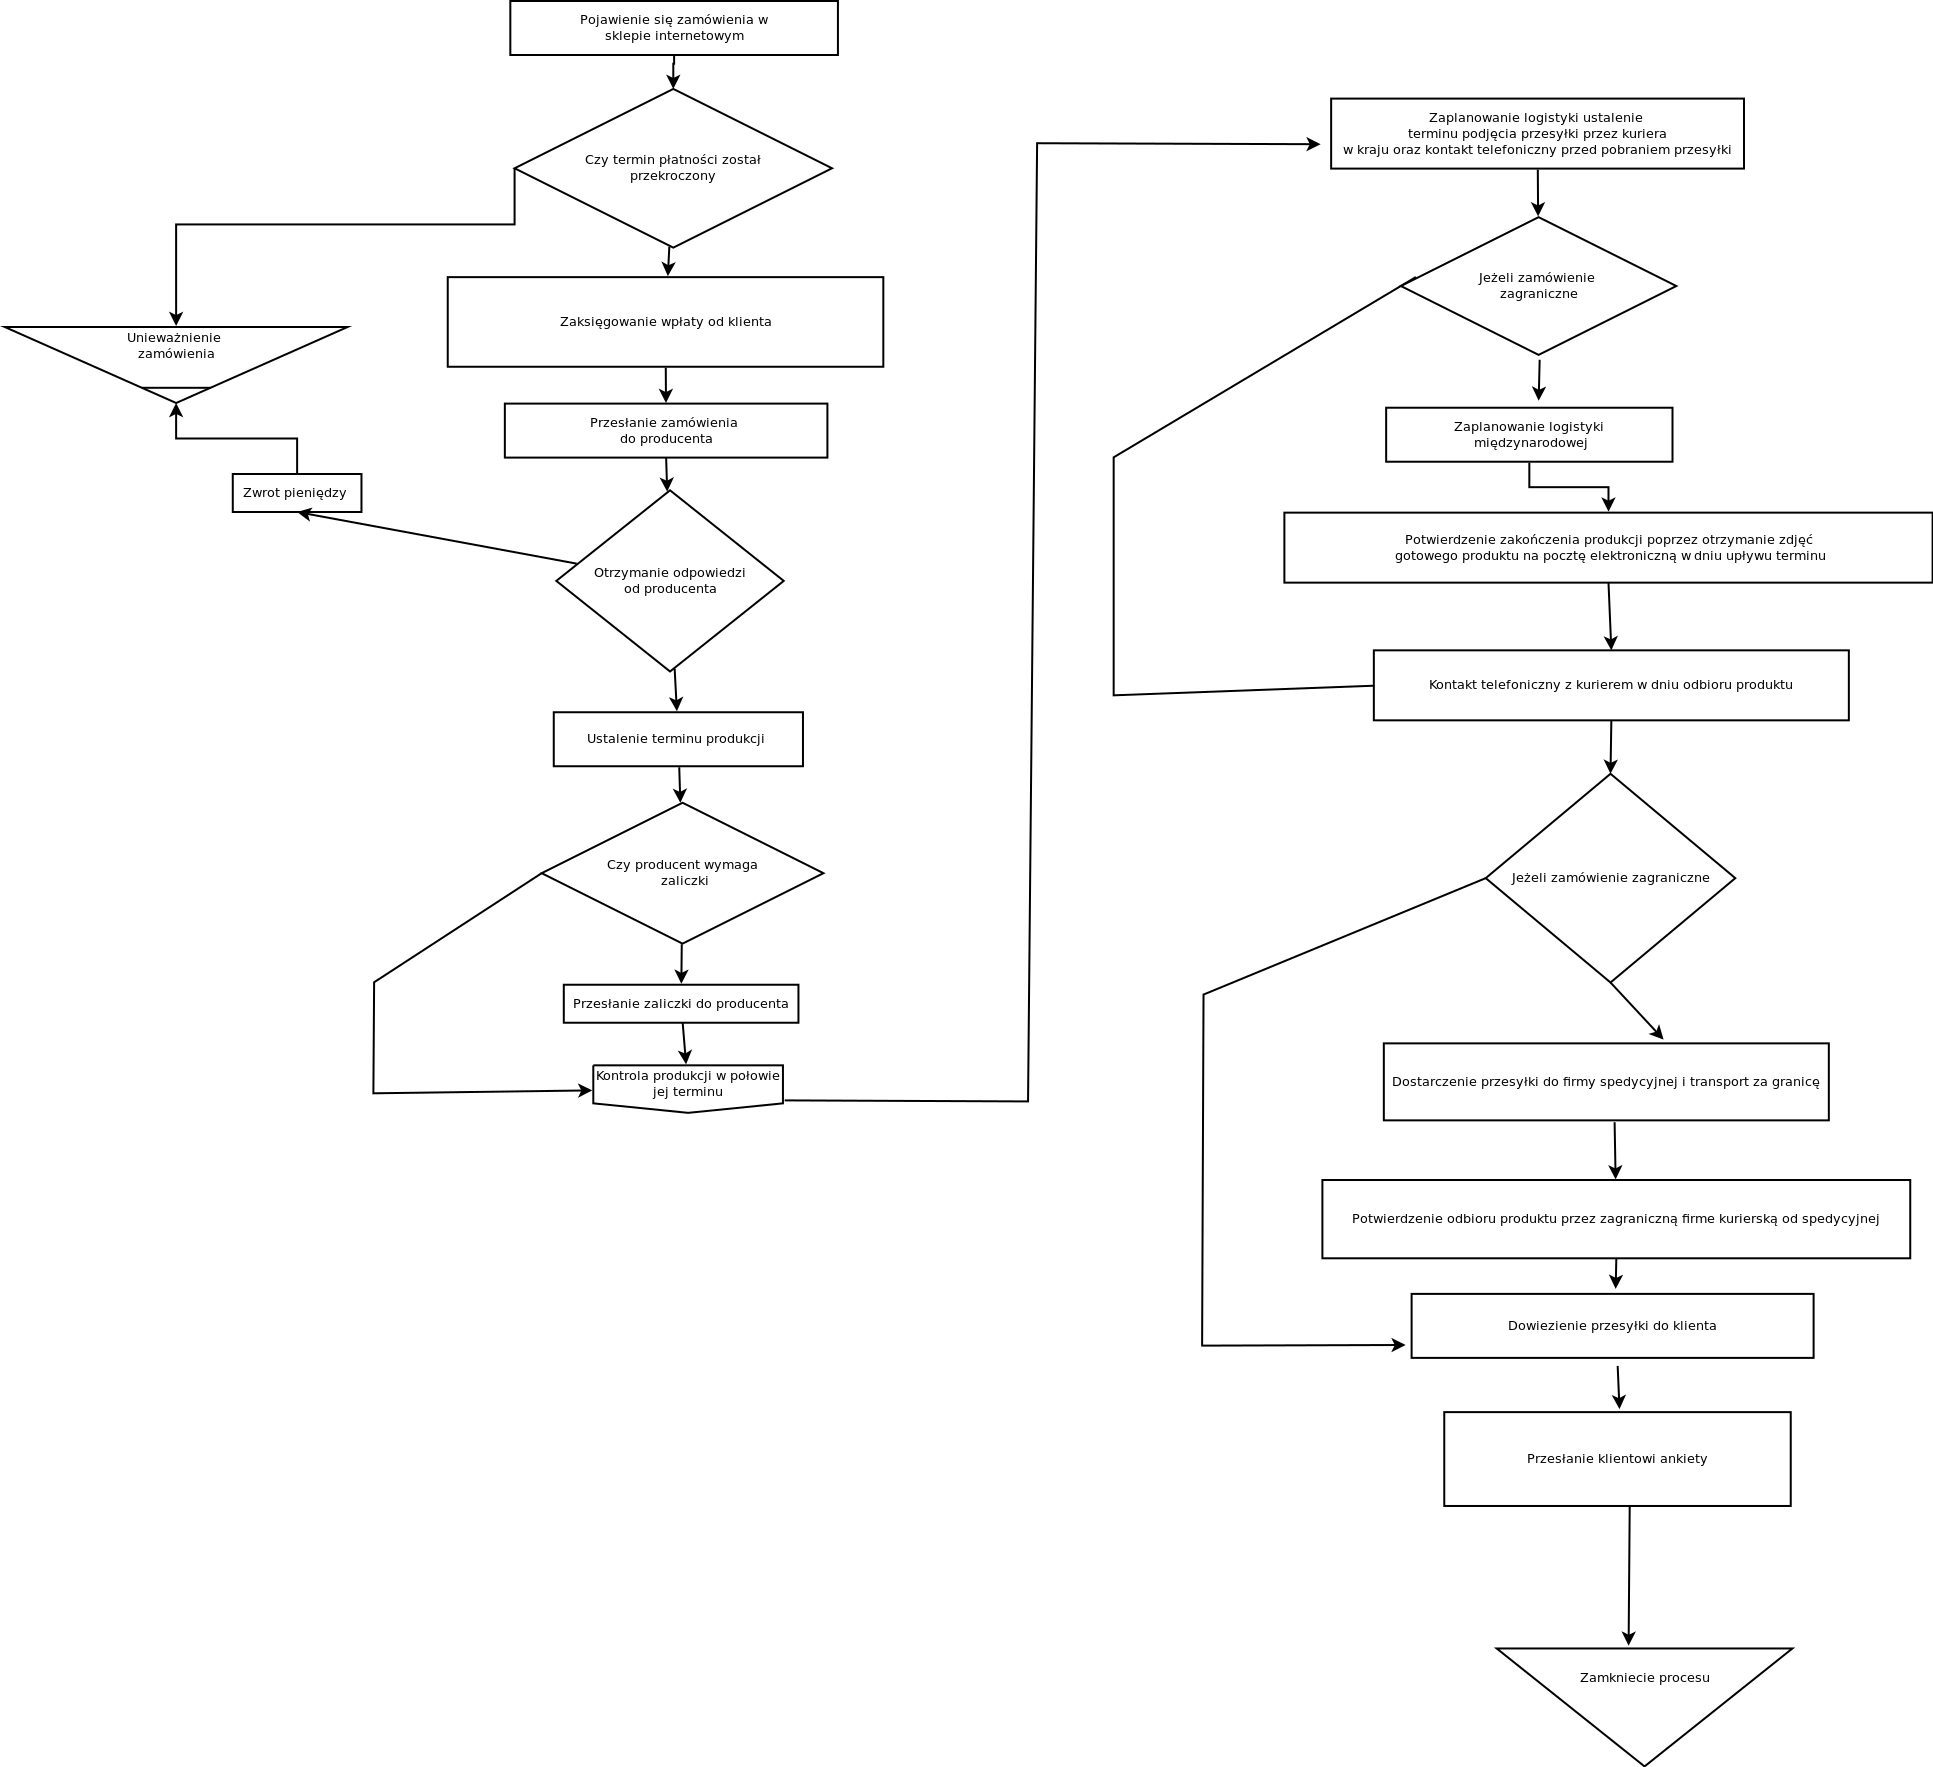
\includegraphics[scale=0.25]{zamowienie}
					\caption{Schemat procesu zamówienia}
				\end{figure}
			
		\subsection{Proces reklamacji}
			\par W tym procesie należy zabezpieczyć dane dotyczące zgłoszenia reklamacji, w skład których muszą wchodzić zdjęcia przedmiotu przesłane przez klienta w zgłoszeniu reklamacji. Na ich podstawie należy podjąć decyzję o uznaniu reklamacji lub odmowie. W wypadku uznania reklamacji i sprzedaży zagranicznej trzeba podjąć odpowiednią procedurę naprawy w kraju docelowym lub wysyłki nowego towaru z Polski i utylizacji uszkodzonego. W wypadku sprzedaży krajowej można zwrócić produkt do producenta celem usunięcia wad.
			
			
			\begin{figure}[H]
				\centering
				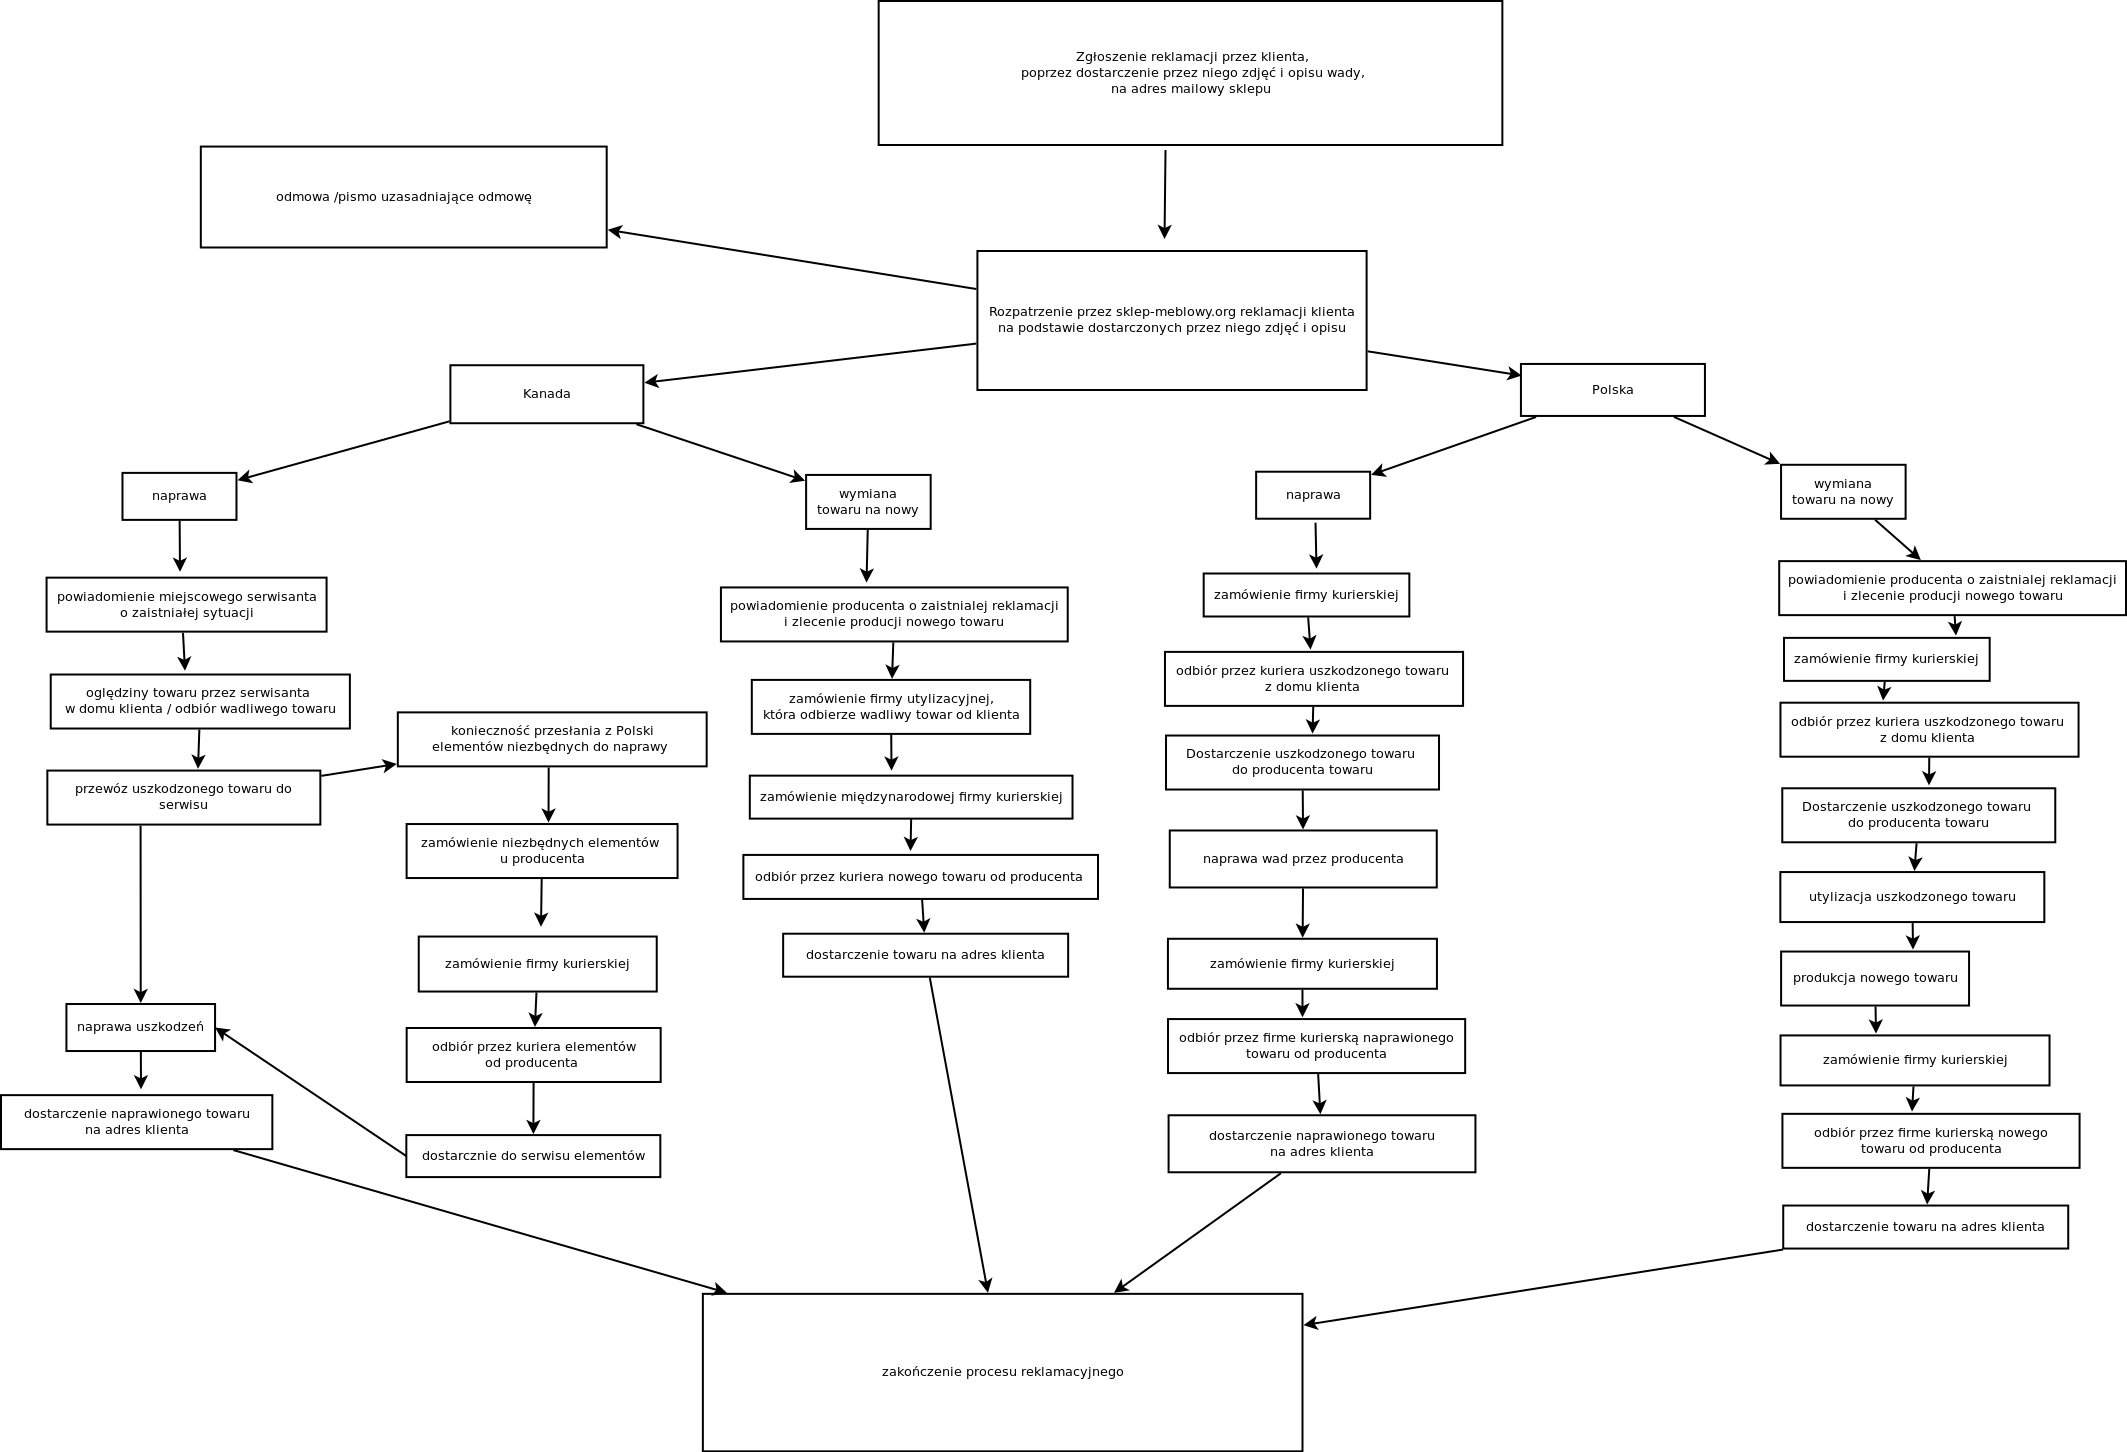
\includegraphics[scale=0.25]{reklamacja}
				\caption{Schemat procesu reklamacji}
			\end{figure}
			

			
			\section{Struktura zatrudnienia i wynagrodzeń}
		\subsection{Opis}
			\par W pierwszym roku prowadzenia działalności mojej firmy będę jej jedynym pracownikiem. Będę odpowiedzialna za pozyskiwanie producentów, których produkty będą prezentowane na stronie, obsługą klientów, logistyką oraz będę się zajmować innymi działaniami niezbędnymi do prowadzenia sklepu internetowego. W trakcie rozwoju firmy planuję zatrudnienie pracowników, którzy przejmą ode mnie część obowiązków. Wprowadzając awanse pionowe, oznaczające pięcie się "w górę" na coraz to wyższe stanowiska w firmie, w drugim roku handlowiec awansuje na stanowisko starszego handlowca, robiąc tym samym lukę, co pozwala na zatrudnienie nowej osoby na stanowisko handlowca. Powielając ten schemat w trzecim roku, starszy handlowiec awansuje na stanowisko kierownika; handlowiec zostanie starszym handlowcem. W ten sposób można zatrudnić kolejną osobę, która zapełni lukę w hierarchii organizacyjnej przedsiębiorstwa. 
			 
			
			\begin{figure}[H]
				\centering
				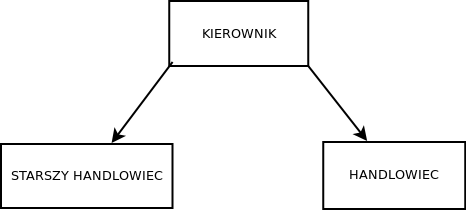
\includegraphics[scale=0.5]{struktura_org}
				\caption{Struktura organizacyjna przedsiębiorstwa}
				\label{search_pl}
			\end{figure}
			
			
		\subsubsection{Opis stanowisk pracy}
			\par Handlowiec
				\begin{itemize}
					\item telefoniczna i mailowa obsługa klienta
					\item obsługa zamówień 
					\item umieszczanie postów na portalach społecznościowych
					\item prowadzenie sprzedaży internetowej poprzez portale aukcyjne
					\item kompletowanie zamówień
			   	\end{itemize}
			
			\par Starszy handlowiec
				\begin{itemize}
					\item umieszczanie nowych produktów na stronie internetowej
					\item sporządzanie szczegółowych opisów produktów
					\item wystawianie faktur, paragonów
					\item kontakt z producentami
					\item kontrola procesu produkcji 
					\item organizowanie logistyki
				\end{itemize}	
					
			\par Kierownik
				\begin{itemize}
					\item pozyskiwanie nowych producentów mebli
					\item kreowanie oraz implementacja rozwiązań, które usprawnią sprzedaż internetową
					\item monitorowanie pracy handlowca i starszego handlowca
					\item monitorowanie rynku i konkurencji
					\item rozpatrywanie reklamacji
					\item delegowanie zadań podległym sobie pracownikom
				\end{itemize}

				
		\subsubsection{Wynagrodzenia}
			\par Przez "wynagrodzenie" rozumiemy ekwiwalent należny za pracę pracownika na rzecz pracodawcy w ramach stosunku pracy. W trakcie rozwoju firmy mam zamiar zatrudniać pracowników na postawie umowy o pracę. Wynagrodzenie początkowe jakie będzie otrzymywał pracownik, to wynagrodzenie minimalne, które zostało ujęte w kodeksie pracy. Na dzień dzisiejszy wynosi ono 2000 zł. brutto. Po otrzymanym awansie, pracownik będzie otrzymywał coraz wyższe wynagrodzenie adekwatne do zajmowanego stanowiska. Można przyjąć, iż będą to podwyżki na poziomie 20-30 \%.
			
			\par Jak powszechnie wiadomo wynagrodzenie pracownika pełni nie tylko funkcję czysto dochodową. Również bardzo ważną jest tu funkcja motywacyjna- im większy wpływ na swoją płacę ma pracownik, tym większą ma motywację do pracy. Dlatego bardzo ważne jest wprowadzenie systemu premii, nagród itp.. W moim przypadku może być to premia związana ze wzrostem sprzedaży, sumienności wykonywanych obowiązków, czy też zaangażowania w rozwój sklepu.

